\documentclass{article}

\usepackage{parskip}
\usepackage{longtable}
\usepackage{pgfplots,subcaption,caption}
\usepackage[justification=centering]{caption}
\usepackage{graphicx,float,amssymb,xcolor}
\graphicspath{ {data/} }
\usepackage{siunitx}
\usepackage{amsmath}

\usepackage{xcolor}
\usepackage{listings}
\usepackage{xparse}
\usepackage{url}

\usepackage{natbib}
\bibliographystyle{apalike}


\setcounter{tocdepth}{3}

\NewDocumentCommand{\codeword}{v}{%
	\texttt{\textcolor{blue}{#1}}%
}

\definecolor{mapgreen}{RGB}{6, 206, 83}
\definecolor{maporange}{RGB}{240, 192, 16}
\definecolor{mapred}{RGB}{255, 1, 1}
\newcommand{\source}[1]{\caption*{Source: {#1}} }

\lstset{language=Python,keywordstyle={\bfseries \color{blue}}}

\usepgfplotslibrary{dateplot}
\pgfplotsset{compat=1.13}

\begin{document}
	\pagenumbering{gobble}

	\begin{titlepage}

		\centering
		\vspace*{-3cm}

		{\scshape\footnotesize Queen Mary, University of London \\ School of Electronic Engineering and Computer Science}

		\vspace{5cm}

		{\huge On-demand forecasting of London crime using PreCrimeBot}


		\vspace{1cm}

		{\large Author: Marcel Tyszkiewicz} \\
		{\small Supervisor: Professor Martin Neil}

		\vspace{10cm}

		{\small April 23, 2018}

	\end{titlepage}

	\begin{abstract}

	\noindent
	For every society known to man, crime has been its constant plague. It is a problem that we have learned to live with, but understand very little of its dynamic. The age of information and technology has not yet provided us with tools that bring us closer to understanding this phenomenon. This project rectifies that by creating a platform that is both easily accessible and one that offers a reliable source of crime likelihood estimation.

	\noindent \\
	Although the main focus of this project will be on an algorithmic solution, crime is a very complex socio-political problem that must be tackled from multiple sides. As discussed later, it is imperative to understand that predictive models inherit bias from their data sources. Obtaining a high predictive accuracy on a dataset cannot therefore accurately capture the complexities of the real world. It is crucial to understand that a lack of variety in data and its sampling has an effect on the final analysis.

	\noindent \\
	I mean to model the underlying crime prediction using a machine learning approach. With industry standard libraries and data from various open sources, I will build a predictive model that will facilitate this forecasting. Using a custom built API, this model can then be coupled with Facebook's Messenger platform by way of a bot integration. This directly solves the underlying problem by allowing anyone with the Messenger app or a browser to instantly access this tool and harness the power of machine learning.

	\end{abstract}

	\newpage
	\renewcommand{\abstractname}{Acknowledgements}

	\begin{abstract}

	\noindent
	The completion of this project would not have been possible without the efforts of many other individuals and groups, whom I would like to sincerely thank before proceeding with this report.


	\noindent \\
	The faculty of the Electronic Engineering and Computer Science at Queen Mary, University of London has been instrumental in aiding my efforts to complete this assignment. From teaching me topics on computation, big data processing and AI, the educational opportunities I received were unparalleled. This education has successfully enabled me to take up further research and study of machine learning, including many advanced algorithmic and mathematical concepts which I relied on to complete this work.

	\noindent \\
	I would specifically like to thank Professor Martin Neil, who has supervised me during my endeavours to complete this project. I would have never reached this stage if not for your extremely useful guidance, which was especially crucial at the early stages of development. I greatly appreciate you devoting your time to supervise me and sharing your immense knowledge in the process. It has been an extremely pleasant experience and one which I will undoubtedly look back on with pleasure.

	\noindent \\
	Lastly, I also owe a debt of gratitude to developers of the Scikit-learn machine learning library. I have based my entire implementation around this fantastic software, which meant I did not have to recreate the wheel when it came to writing classifiers and could focus my efforts on other tasks. Its superbly well designed API and descriptive examples were very refreshing and pleasant to work with.
	\end{abstract}


	\newpage
	\pagenumbering{arabic}

	\tableofcontents
	\newpage

	\section{Introduction}

	\subsection{Problem statement}

	My primary interest is in analysing crime patterns and other factors that might have an impact on crime. Crucially, the results of this analysis should be universally accessible without the need for sophisticated software or expert knowledge.

	Whilst crime and forecasting are fairly short and concise terms, they are a facade to two very complex processes. Due to time and other practical limitations, this project implements only one of many possible ways of modelling these processes, however several proposals will be made as to how this could be extended in the future.

	It is worth noting that there is a multitude of ways to approach this problem and many such solutions have been implemented at scale for law enforcement and government agencies. No quality solution exists for the public, however.

	Inspired by the film Minority Report, this platform is meant to be a gateway that allows on-demand access to predictions of crime in London. This could have various potential applications, from making travel plans to deciding which property to buy. Of course, there are legitimate business use cases for this tool, such as insurance companies and banks looking to invest or insure, or even police forces looking to target specific crime hot zones.

	\subsection{Proposed approach}

	As an answer to the above problem, this project focuses on a machine learning solution that can be easily queried to forecast crime. This implementation is limited to the London area, however this could easily be expanded nationally or internationally with the right data sources.

	Since a large part of this project is to make this platform as accessible as possible, I have opted to integrate it with Facebook Messenger. Its user base now totals over 1.2 billion, making it one of the most widespread in the world. As various industries are now rushing to expose their products on this platform, it seemed only logical to the same. A Messenger Bot integration means that those 1.2 billion users can interact with my predictive model without having to install any additional software (assuming they already have the Messenger app or a browser).



	\section{Implementation}

	\subsection{Software stack}

	\subsubsection{Programming language}

	One of the first and most crucial considerations I had to make was choosing a programming language to work with. My main point of focus was to choose a language that has a rich offering of machine learning libraries and that is easy to work with. For this reason I have chosen to use Python, a language I had experience with and know to be both cross-platform and well suited to the task.

	\subsubsection{Frameworks and libraries}
	Other than my familiarity with Python, I was extremely impressed with the Scikit-learn library, which is an open source library specifically designed for machine learning tasks. Its concise documentation, plentiful examples and its extremely thorough review by \cite{sklearn_api} convinced me to rely on it in this project.

	In addition to Scikit-learn, Python has a wide range of modules and libraries for other common tasks. Many of these I use in my project, namely:

	\begin{itemize}
		\item Flask, a micro framework for writing HTTP applications,
		\item GeoPy, an address geocoding client,
		\item dateparser, a module for parsing human readable dates,
		\item Pandas, a data manipulation and analysis library,
		\item NumPy, a library for large scale matrix manipulation and arithmetic operations,
		\item Python Prompt Toolkit, a library for building interactive command line interfaces.
	\end{itemize}

	\subsubsection{MySQL and QGIS as data analysis tools}

	Visualising textual data is something humans are awful at, so to analyse the available datasources I decided to use specialised software.

	QGIS is an open-source geographic information system for viewing of geospatial data. This software has enabled me understand the data I am dealing with by superimposing it on various maps, some of which I include in this report.

	Other than a geographic understanding of data, it is also crucial to analyse it from a statistical perspective. This involves using aggregation and arithmetic methods, as well as filtering and sorting. The tool that I immediately thought of for this task is a relational database, as I am quite proficient with SQL. I chose to use a MySQL database for this purpose.

	\subsection{Data}

	\subsubsection{Understanding bias}

	Before explaining exactly which data sources I have decided to use, it is imperative to talk about data bias and the role it plays in any algorithmic analysis.

	To understand bias, we must remember that all machine learning algorithms are powered by the data they are given. This might seem fairly obvious, but what is not always obvious, however, is that all data is inherently biased, as it only paints one narrow part of the bigger picture. Unless we can provide an algorithm with a dataset that perfectly models the entire universe, then we will never have a complete model.

	Let me illustrate this using practical examples. You might have heard the rhetorical question that a parent asks their child: "if all your friends jumped off a bridge, would you follow them?". A machine learning algorithm would say: "yes, definitely". Models, just like pets, have to be trained to avoid certain situations, they have no built-in cognition that will tell them to avoid danger. Now let us consider one of humanity's greatest achievements, landing on the Moon. Of the twelve people that ever walked the planet, all were middle-aged, white, American males. A model trained on this data alone would never predict a person of another sex or race reaching the planet. While these examples are extreme, they illustrate the problem of any predictive tool. It is perfectly reasonable to expect a person of another race or gender to walk on the Moon some day. It is also possible that we were jumping off the bridge with a parachute and would be safe from harm. But neither of these facts was included in the data.

	A recent Nature article by \cite{shapiro} raises questions about making direct links between complex events like crime and shallow properties like time, location or even temperature. An important point is also raised about the existence of a connection between the race and the socio-economic status of inhabitants of certain geographical locations. An analysis that predicts more crime in that zone carries an implicit declaration about those individuals and their status in society. Crime reports, in particular, are directly linked to policing patterns; deploying more officers to a location will mean more crime reports in that zone and conversely, less in others. Furthermore, some individuals are less likely to report crimes, which further skews the results.

	Not all of these problems can be easily addressed, but one way to help alleviate bias is to use more data sources. A plethora of factors play a part in what happens around us, from weather patterns to how well one's favourite football team is faring. Some of those are easier to model than others, however incorporating as many features as possible into the model will mean we can study those complex relationships.

	In this implementation I have chosen to limit myself to only one datasource. This was a conscious decision made due to time and cost considerations. In a real-world application, however, this shallow representation of the world using a single source of data would not suffice. In the future improvements section of this report I outline this as a possible improvement.

	\subsubsection{Data source: UK Police open crime data}

	The Home Office publishes historical data about crimes collected from 43 police forces across the United Kingdom. At the time of writing, this dataset spans a period from December 2014 to November 2017.

	Given that it seems to be the most relevant source to the task at hand, this is the dataset I decided to use in my project. This decision, however, has placed some limitations on my implementation.

	Due to privacy and anonymity concerns, all timestamps are truncated to the year and month of occurrence. Additionally, all locations are skewed so that they:

	\begin{itemize}
		\item have a catchment area of at least eight postal addresses or none at all,
		\item appear over one of:
		\begin{itemize}
			\item the centre of a street,
			\item a public place, such as a park or airport,
			\item a commercial premises, such as a shopping centre or nightclub.
		\end{itemize}
	\end{itemize}

	This means that, at best, a trained model could only make monthly predictions limited to a geographical radius, not a particular day or location. As there is no alternative source of crime information that covers the UK, I have decided to accept this anonymised dataset as a source of truth in my implementation.

	Through the government open data portal, this dataset has been made available for download in the form of CSV files. This makes it extremely convenient to train models on, as there was no need to perform API scraping.

	Of the entire dataset, I have chosen to limit it to the two London police forces, the Metropolitan Police Service (MPS) and City of London Police. This 36 month dataset contains a total of 2,996,065 records which, when uncompressed on the disk, take up just short of 700MB of space. The size of this dataset meant I could train the models locally without the need for any clustered processing.

	Table \ref{fig:field-description} shows a definition of all attribute columns contained in this dataset.

	\begin{longtable}{p{2.2cm}p{7.8cm}}
		\caption{Description of crime attributes \\ Source: www.police.uk}
		\label{fig:field-description} \\
		\hline
		{\bf Attribute name} & {\bf Description} \\ \hline
		\endhead
		Month & A YYYY-MM formatted timestamp, e.g. 2017-10 \\ \hline
		Reported by, Falls within & Name of the force that provided the data about the crime \\ \hline
		Longitude, latitude & Anonymised coordinates \\ \hline
		Location & Description of nearest street, park or other public location \\ \hline
		LSOA code, LSOA name & References to the Lower Layer Super Output Area boundaries (administrative zones within the UK) \\ \hline
		Crime type & One of 15 predefined crime categories \\ \hline
		Last outcome category & Reference to the outcome of the last action on file for this crime, e.g. "investigation complete" \\ \hline
		Context & Human readable description \\ \hline
	\end{longtable}

	Table \ref{fig:category-description} includes a detailed explanation of which categories each crime is classified into. Each crime instance is attributed to exactly one category. This makes many machine learning tasks a lot easier, as multi-label problems can be difficult to work with.

	\begin{longtable}{p{2.2cm}p{7.8cm}}
		\caption{Description of crime categories \\ Source: www.police.uk}
		\label{fig:category-description} \\
		\hline
		{\bf Category} & {\bf Description} \\ \hline
		\endhead
		Anti-social behaviour & Includes personal, environmental and nuisance anti-social behaviour \\ \hline
		Bicycle theft & Includes the taking without consent or theft of a pedal cycle \\ \hline
		Burglary & Includes offences where a person enters a house or other building with the intention of stealing \\ \hline
		Criminal damage and arson & Includes damage to buildings and vehicles and deliberate damage by fire \\ \hline
		Drugs & Includes offences related to possession, supply and production \\ \hline
		Other crime & Includes forgery, perjury and other miscellaneous crime \\ \hline
		Other theft & Includes theft by an employee, blackmail and making off without payment \\ \hline
		Possession of weapons & Includes possession of a weapon, such as a firearm or knife \\ \hline
		Public disorder and weapons & Includes offences which cause fear, alarm, distress or a possession of a weapon such as a firearm \\ \hline
		Public order & Includes offences which cause fear, alarm or distress \\ \hline
		Robbery & Includes offences where a person uses force or threat of force to steal \\ \hline
		Shoplifting & Includes theft from shops or stalls \\ \hline
		Theft from the person & Includes crimes that involve theft directly from the victim (including handbag, wallet, cash, mobile phones) but without the use or threat of physical force \\ \hline
		Vehicle crime & Includes theft from or of a vehicle or interference with a vehicle \\ \hline
		Violence and sexual offences & Includes offences against the person such as common assaults, Grievous Bodily Harm and sexual offences \\ \hline
	\end{longtable}

	\subsubsection{Statistical analysis}

	After completing the preliminary analysis of the available data, I then proceeded to load all the records into a MySQL database. This allowed me to use its powerful SQL engine to get a deeper understanding of the underlying data, as well as its trends.

	Figure \ref{fig:crime-distribution} shows how the fifteen crime categories are distributed in frequency of their occurrence. Rather unexpectedly, it is anti-social behaviour that is reported most frequently, while possession of weapons is on the opposite end of the scale.

	This data accounts for the entire 36 month period for both London police forces, so we should expect similar results in our final model.

	\begin{figure}[H]
		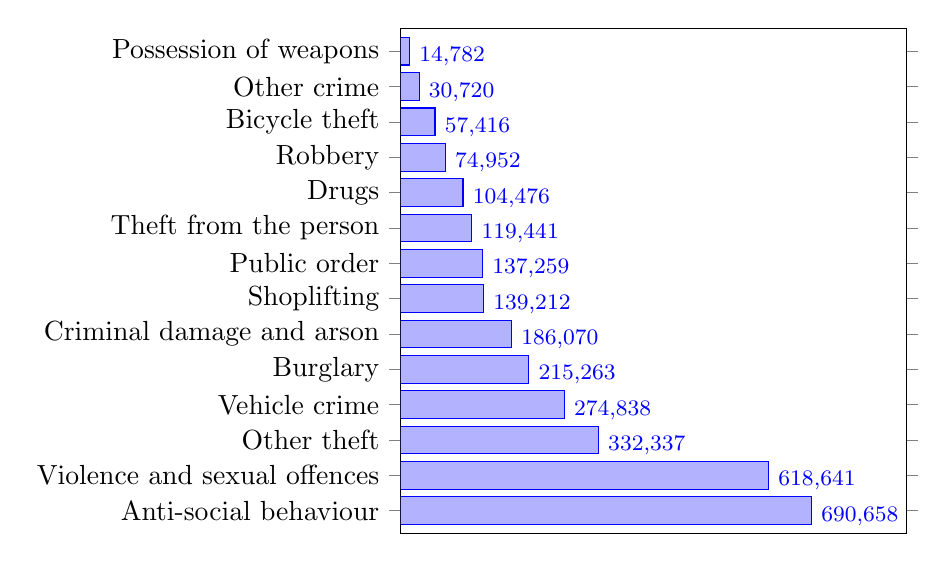
\begin{tikzpicture}
			\begin{axis}[
				xbar,
				xmin=0,
				xmax=850000,
				width=8cm,
				height=8cm,
				enlarge y limits=0.05,
				symbolic y coords={
					Anti-social behaviour,
					Violence and sexual offences,
					Other theft,
					Vehicle crime,
					Burglary,
					Criminal damage and arson,
					Shoplifting,
					Public order,
					Theft from the person,
					Drugs,
					Robbery,
					Bicycle theft,
					Other crime,
					Possession of weapons,
				},
				ytick=data,
				xtick=\empty,
				nodes near coords,
				every node near coord/.append style={
					/pgf/number format/fixed,
					/pgf/number format/precision=5,
					yshift=-2pt,
					font=\footnotesize,
				},
			]
				\addplot coordinates {
					(690658,Anti-social behaviour) (57416,Bicycle theft) (215263,Burglary)
					(186070,Criminal damage and arson) (104476,Drugs) (30720,Other crime)
					(332337,Other theft) (14782,Possession of weapons) (137259,Public order)
					(74952,Robbery) (139212,Shoplifting) (119441,Theft from the person)
					(274838,Vehicle crime) (618641,Violence and sexual offences)
				};
			\end{axis}
		\end{tikzpicture}
		\caption{Distribution of crime occurrences in each category}
		\label{fig:crime-distribution}
	\end{figure}

	Figure \ref{monthly-crime-occurrences} shows the monthly number of reported crimes during this period. This number has stayed reasonably even, with an average of 83,224 occurrences per month and a standard deviation of 6,772. The lowest number of observed crime was in February 2015 with 69,311 reports, while the highest occurred in July 2017 with 96,857 reports.

	\begin{figure}[H]
		\centering
		\begin{tikzpicture}
			\begin{axis} [
				ymin=0,
				width=0.8\textwidth,
				ymax=100000,
				ytick distance=20000,
				height=5.5cm,
				date coordinates in=x,
				enlarge x limits=false,
				ylabel=Number of occurrences,
				xlabel=Time period,
				xlabel style={color=gray},
				ylabel style={color=gray},
				xtick distance=120,
				xticklabel={\month-\year},
				xticklabel style={rotate=45,xshift=-8pt,yshift=8pt},
				scaled y ticks=false,
				every axis plot/.append style={thick},
				yticklabel style={
					/pgf/number format/fixed,
					/pgf/number format/precision=5
				},
			]
				\addplot [smooth,blue] table [x=date,y=count,col sep=comma] {data/count-grouped-by-date.csv};
			\end{axis}
		\end{tikzpicture}
		\caption{Monthly number of crime occurrences}
		\label{monthly-crime-occurrences}
	\end{figure}

	It is also clear that there is an obvious spike around July of each year. Additionally, we can see that there is a trend for the number of reported crimes to grow with the passage of time. This becomes more clear in figure \ref{monthly-crime-closer}, which is asymmetrically scaled.

	\begin{figure}[H]
		\centering
		\begin{tikzpicture}
			\begin{axis} [
				width=0.8\textwidth,
				height=5.5cm,
				ymax=100000,
				ytick distance=10000,
				date coordinates in=x,
				enlarge x limits=false,
				ylabel=Number of occurrences,
				xlabel=Time period,
				xlabel style={color=gray},
				ylabel style={color=gray},
				xtick distance=120,
				xticklabel={\month-\year},
				xticklabel style={rotate=45,xshift=-8pt,yshift=8pt},
				scaled y ticks=false,
				every axis plot/.append style={thick},
				yticklabel style={
					/pgf/number format/fixed,
					/pgf/number format/precision=5
				},
			]
				\addplot [smooth,blue] table [x=date,y=count,col sep=comma] {data/count-grouped-by-date.csv};
			\end{axis}
		\end{tikzpicture}
		\caption{Monthly number of crime occurrences}
		\label{monthly-crime-closer}
	\end{figure}

	In addition to the spike around July, we also observe a drop in crime in February. It is very interesting to see this pattern so clearly defined on an annual basis. Further deductions about this phenomenon would require an analysis of historical data reaching at least a few decades back. It is very possible, however, that this seasonality is caused by weather patterns. It could be very beneficial to introduce meteorological data into the model, which is mentioned in the future improvements section of this report.

	\subsubsection{Graphical analysis}

	Having understood the size of the dataset I was dealing with, as well as its trends, I then proceeded to analyse the data graphically using QGIS.

	First I began by superimposing the entire 36 month crime dataset onto a map of the United Kingdom (fig. \ref{fig:map-whole}).

	Interestingly none of the crime reports contained any locations in Scotland or Northern Ireland (removed from map in fig. \ref{fig:map-whole}). This is most likely due to reporting or jurisdictional procedures rather than a natural lack of crime in those regions.

	This form of data analysis helped me correct an assumption I had made about the data only referencing locations within the London area. The crime locations could be arbitrary, it is the reporting police force that is the key factor here.

	\begin{figure}[H]
		\centering
		\includegraphics[width=7.6cm]{crime-map.png}

		\scriptsize
		\hfill

		\fbox{\begin{tabular}{ll}
				\textcolor{mapred}{$\blacksquare$} & M25 motorway \\
				\textcolor{mapgreen}{$\blacksquare$} & Metropolitan Police reports \\
				\textcolor{maporange}{$\blacksquare$} & City of London Police reports \\
		\end{tabular}}
		\caption{Mapping of the entire crime dataset}
		\label{fig:map-whole}
	\end{figure}

	Given that I only wish to forecast crime that occurs in London, this poses two dilemmas. Firstly, the City of London and MPS crime datasets contain information about crimes that did not occur in London. Secondly, datasets for other police jurisdictions may contain information crimes that did occur in London.

	The first of these issues I address in the process of feature engineering, as outlined in the next section.

	Addressing the second dilemma would involve parsing all of the crime datasets that the government publicises and extracting those that occurred in London. This is relatively simple from a programmatic perspective, however requires fairly large computational resources and I felt that it would not add enough value to this project. I have therefore decided to stick with the MPS and City of London datasets alone.

	\subsection{Use cases}

	The current design of this application is extremely straightforward and thus includes only one use case. That is to allow users to ask for predictions based on some arbitrary location and time. The returned result should be a list of crime categories along with their predicted probability of occurrence.

	It is important that both the address and location parameters are lax enough to accept different formats, including human readable and computer formatted values.

	Additionally, there should be ways to use this tool in programmatic environments (e.g. in a program or script).

	\subsection{Feature engineering}

	After having chosen the UK Police dataset to address the problem at hand, I began the process of feature extraction for model training. As per the use cases mentioned before, the three attributes that jumped out were:

	\begin{enumerate}
		\item month,
		\item longitude,
		\item latitude,
		\item crime type.
	\end{enumerate}

	The last attribute would, of course, be the target label.

	Having assembled these four features to use in training, I was now ready to start the data preprocessing phase. This is a necessary step to ensure that machine learning models yield a high predictive accuracy whilst maintaining a reasonable training time.

	\subsubsection{Preprocessing}

	Of the entire UK Police dataset, I only chose the subset that pertains to the Metropolitan and City of London police forces. Combined they have a catchment area of \SI{1580}{\kilo\metre\squared}. Additionally, each instance row is attributed to one of fifteen crime categories.  This poses many problems for a machine learning model which aims to find links between related features. If there are too many of those features, or they take too many values, then the model will not be able to generalise well enough to make those associations.

	As a result of the above statistical and geographical analysis outlined above, I was able to pinpoint the following major problems with the source data:

	\begin{enumerate}
		\item There are too many target labels (crime categories), which could negatively influence the resulting model. As shown previously, some of the categories are disproportionally larger than others, meaning they exhibit a tendency to dominate.
		\item Many of the reports are localised outside of the London area of interest.
		\item The date of each event is represented as a compound month-year attribute, which will prevent the model from noticing monthly trends.
		\item The dataset contains approximately 65,000 distinct coordinate pairs. This introduces unneeded complexity into the model, as we do not need to make predictions for specific locations.
		\item Some reports do not have an associated latitude and longitude coordinate pair.
	\end{enumerate}

	To alleviate these issues, I came up with the following strategies:

	\paragraph{Reducing target labels}

	After having studied the crime categories and their descriptions, I was able to use domain knowledge to merge the fifteen crime categories into three. This new mapping is explained in table \ref{tab:new-target-labels}.

	\begin{longtable}{|p{1.8cm}|p{7cm}|p{1.8cm}|}
		\caption{Merged crime categories \\ Source: www.police.uk}
		\label{tab:new-target-labels} \\
		\hline
		{\bf Original category} & {\bf Description}  & {\bf Merged category} \\ \hline
		\endhead
		Bicycle theft & Includes the taking without consent or theft of a pedal cycle & Theft \\ \hline
		Shoplifting & Includes theft from shops or stalls & Theft \\ \hline
		Burglary & Includes offences where a person enters a house or other building with the intention of stealing & Theft \\ \hline
		Theft from the person & Includes crimes that involve theft directly from the victim but without the use or threat of physical force & Theft \\ \hline
		Vehicle crime & Includes theft from or of a vehicle or interference with a vehicle & Theft \\ \hline
		Other theft & Includes theft by an employee, blackmail and making off without payment & Theft \\ \hline
		Possession of weapons & Includes possession of a weapon, such as a firearm or knife & Serious crime \\ \hline
		Public disorder and weapons & Includes offences which cause fear, alarm, distress or a possession of a weapon such as a firearm & Serious crime \\ \hline
		Criminal damage and arson & Includes damage to buildings and vehicles and deliberate damage by fire & Serious crime \\ \hline
		Violence and sexual offences & Includes offences against the person such as common assaults, Grievous Bodily Harm and sexual offences & Serious crime \\ \hline
		Robbery & Includes offences where a person uses force or threat of force to steal & Serious crime \\ \hline
		Anti-social behaviour & Includes personal, environmental and nuisance anti-social behaviour & Minor and other crime \\ \hline
		Drugs & Includes offences related to possession, supply and production & Minor and other crime \\ \hline
		Public order & Includes offences which cause fear, alarm or distress & Minor and other crime \\ \hline
		Other crime & Includes forgery, perjury and other miscellaneous crime & Minor and other crime \\ \hline
	\end{longtable}

	At this point I went back a few steps to analyse how this new classification works in practice. Figure \ref{fig:distribution-new} shows that the number of instances within each new class is now much more evenly distributed. Theft accounts for 38\% of all instances, while serious and other crime account for 30\% and 32\%, respectively.

	\begin{figure}[H]
		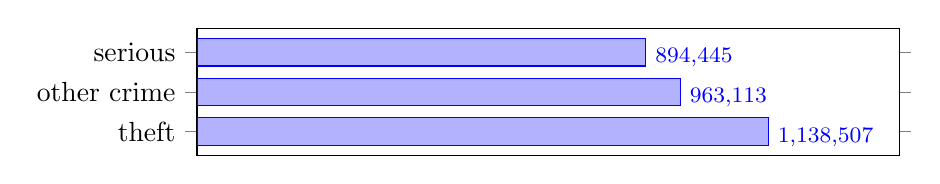
\begin{tikzpicture}
		\begin{axis}[
		xbar,
		xmin=0,
		xmax=1400000,
		width=10.5cm,
		height=3.2cm,
		enlarge y limits=0.3,
		symbolic y coords={theft,other crime,serious},
		ytick=data,
		xtick=\empty,
		nodes near coords,
		every node near coord/.append style={
			/pgf/number format/fixed,
			/pgf/number format/precision=5,
			yshift=-2pt,
			font=\footnotesize,
		},
		]
		\addplot coordinates {(1138507,theft) (894445,serious) (963113,other crime)};
		\end{axis}
		\end{tikzpicture}
		\caption{Distribution of crime occurrences in each new category}
		\label{fig:distribution-new}
	\end{figure}

	It is also interesting to see the relationship exhibited by these new categories on a monthly basis. Figure \ref{fig:distribution-new-compared} allows us to observe a pattern between the reports of theft and serious crimes. The crimes that fall into the "other" category appear to be a bit more seasonal, with definite spikes in the summer months, reaching an extreme in July of 2016.

	\begin{figure}[H]
		\centering
		\begin{tikzpicture}
		\begin{axis} [
		ymin=0,
		width=10cm,
		height=6cm,
		enlarge x limits=false,
		date coordinates in=x,
		ylabel=Number of occurrences,
		xlabel=Time period,
		xlabel style={color=gray},
		ylabel style={color=gray},
		xtick distance=120,
		xticklabel={\month-\year},
		xticklabel style={rotate=45},
		legend style={
			area legend,
			at={(0.5,0.2)},
			anchor=north,
			legend columns=-1,
		},
		scaled y ticks=false,
		every axis plot/.append style={thick},
		]
		\addplot [smooth,blue] table [x=date,y=theft,col sep=comma] {data/count-for-each-category-and-month.csv};
		\addplot [smooth,teal] table [x=date,y=serious,col sep=comma] {data/count-for-each-category-and-month.csv};
		\addplot [smooth,orange] table [x=date,y=other,col sep=comma] {data/count-for-each-category-and-month.csv};
		\legend {theft,serious,other}
		\end{axis}
		\end{tikzpicture}
		\caption{Monthly crime occurrences for each new category}
		\label{fig:distribution-new-compared}
	\end{figure}

	\paragraph{Excluding reports without a location}

	I have implemented a module called \codeword{data_loader} which, as the name suggests, is responsible for loading data into the application. In it I make heavy use of the Pandas module for parsing and handling CSV files.

	Once a CSV is read from the disk and parsed, it is represented as a \codeword{dataframe} object. This object exposes a plethora of manipulation methods, including those that allow for filtering based on cell values. I use these to exclude any rows (instances) that do not include a latitude or longitude coordinate.

	\paragraph{Excluding non-relevant locations}

	Given that the focus area of this project is to forecast London crime, any reports that fall outside of this region are anomalies that will distract the model. Before these anomalies can be dealt with, however, it is important to answer one question: where exactly does London start/end?

	A potential solution could be to reverse geocode each coordinate to produce an address, then checking whether that address falls within London. The problem with this approach, however, is that reverse geocoding involves an external HTTP request for each coordinate pair, which would lead to a very significant delay given the dataset size.

	Another solution, which is the one I ended up employing, is to use a geographical boundary as a catchment area. For this purpose I used the M25 motorway, excluding all locations that fall outside of it. From a computational perspective this approach is much faster as it reduces to a simple problem: figuring out whether a given point is within a certain polygon.

	Before proceeding any further, I had to obtain the coordinates for identifying points of the M25 to define that outer polygon. I store these in a JSON file within the application, which I then load in my \codeword{location_filtering} module. Next, using the Shapely Python package, I convert these points into a \codeword{Polygon} object which exposes a \codeword{contains(point)} method. I wrapped all this up in a convenient \codeword{is_within_m25(lat, lon)} method that can be easily reused to filter out locations based on this criterion.

	This process excluded 38,804 anomalies, leaving us with a total of 2,957,326 instances, of which 2,939,666 were reported by the MPS and 17,660 by the City of London Police. Figure \ref{fig:map-filtered} shows these points superimposed onto a map of the M25 area.

	\begin{figure}[H]
		\centering
		\includegraphics[width=10cm]{crime-map-filtered.png}

		\scriptsize
		\hfill

		\fbox{\begin{tabular}{ll}
			\textcolor{mapred}{$\blacksquare$} & M25 motorway \\
			\textcolor{mapgreen}{$\blacksquare$} & Metropolitan Police reports \\
			\textcolor{maporange}{$\blacksquare$} & City of London Police reports \\
		\end{tabular}}
		\caption{Mapping of the crime dataset, narrowed to the M25 area}
		\label{fig:map-filtered}
	\end{figure}

The map in fig. \ref{fig:map-filtered} also shows the coordinates that were used as outer bounds of the M25 motorway. They do not form a perfect overlay of the road, as only 53 coordinates were used, however this precision is satisfactory for the implementation at hand. If it were a requirement to detect locations with perfect precision, then using the Ordnance Survey mapping APIs would be a better alternative, however it introduces the same HTTP overhead as mentioned before.

	\paragraph{Separating compound attributes}

	Using Python's \codeword{datetime} module I separate the compound \codeword{YYYY-MM} formatted date into two features: month and year. This is done automatically by my \codeword{data_loader} module whenever a CSV file is parsed.

	\paragraph{Merging related locations}

	As coordinates represent geographical locations, they lend themselves quite well to distance-based comparisons. While this is an ideal feature for machine learning, it is far from ideal for them to take nearly 65,000 values.

	Initially I had two ideas: to divide London into regions using a grid-based approach or by grouping together London's boroughs. Both of these approaches, however, have their disadvantages. Most importantly they require additional work and expert knowledge of the area, but also they both introduce very rigid regions that may not naturally correlate with what is in the input dataset. Essentially these approaches would divide London into regions, whereas we are aiming to divide the crime instances into their own regions. The two, whilst geographically similar, may be disparate.

	Using a clustering algorithm, such as K-means, alleviates both of these issues. This algorithm takes as input a list of points and a number of clusters (regions) to divide them into, and produces a list of centroids (centre points) for those newly formed clusters. This means that we can easily change the number of regions we want to create and that we can easily implement this solution without any expert knowledge.

	The clustering solution is the one I opted for in the end, choosing to divide the input crime instances into 20 distinct regions using the Scikit-learn library. Before training the model on any new data I dynamically swap the latitude and longitude columns with the correct cluster index. This logic is placed within my \codeword{data_loader} module. Figure \ref{fig:map-centroid} shows the locations of these centroids as well as their relative size, based on the number of points within that cluster.

	\begin{figure}[H]
		\centering
		\includegraphics[width=10cm]{centroid-map.png}

		\scriptsize
		\hfill

		\fbox{\begin{tabular}{ll}
				\textcolor{mapred}{$\blacksquare$} & M25 motorway \\
				\textcolor{blue}{$\blacksquare$} & Centroids \\
		\end{tabular}}
		\caption{Mapping of cluster centroids with relative size}
		\label{fig:map-centroid}
	\end{figure}

	\subsection{Classifier comparison}

	The target use case of this prediction engine is to forecast probabilities of crime occurrence based on certain attributes. The target label (crime category) is known and the dataset maps all attributes to this label, therefore this is a supervised learning problem.  Additionally, the target label is discrete, so this is a classification problem with a slight twist - we want to predict class probabilities, not the classes.

	The Scikit-learn library is extremely well suited to this task, as it provides a wide range of classifier implementations, namely:

	\begin{itemize}
		\item Artificial Neural Networks,
		\item Random Forests,
		\item Logistic Regression (Max Entropy),
		\item Stochastic Gradient Descent.
	\end{itemize}

	The difficulty is that the source dataset contains nearly 3 million instances with the following 4 attributes:

	\begin{enumerate}
		\item month,
		\item year,
		\item location,
		\item crime category.
	\end{enumerate}

	Moreover, some of the models work better with data that uses one-hot encoding. In this case it would mean swapping the location attribute (which takes one of 20 integer values) with 20 attributes, thus raising the amount of attributes from 4 to 23.

	To pick the best model it is therefore critical to consider two things:

	\begin{enumerate}
		\item The performance aspects of the above classifiers and how they will scale in terms of input.
		\item Which meaningful metric we can use to rank them and choose the best one.
	\end{enumerate}

	\subsubsection{Accuracy metrics}

	When performing any machine learning task, it is important to be able to assign a meaningful score to the predicted result. This offers a way of calibrating models and having some degree of confidence in the learned model.

	\paragraph{Subset classification as a metric}

	For classification tasks the go-to metric is the number of correctly classified instances. This is usually fine, however we are faced with a multi-class classification problem with a dataset of 3 million records, of which I use 90\% for training. To rate the classifier I would then have to test how many of the approximately 300,000 test instances it classed correctly.

	Given the scale and multi-class nature of the problem, this is an incredibly harsh metric. If the classifier were random, then we could hope for an average accuracy of 33\%, since we only have 3 distinct target labels.

	\paragraph{Mean absolute percentage error (MAPE) as a metric}

	Considering the intended use case of this application (to estimate probability distributions, not to classify directly), using the subset classification metric is far from ideal. Ideally we would like to score the classifiers based on the probability estimates that they provide, not the classification prediction.

	One such metric is called mean absolute percentage error (MAPE) and it is both much more intuitive and one that is designed for comparing percentage values (\cite{MAPE}). This metric compares all the predicted probability values to the actual probabilities and returns their mean.

	\begin{figure}[H]
		\begin{equation}
			MAPE = \frac{1}{n} * \sum\limits_{i=1}^n \frac{|observed - predicted|}{|observed|}
		\end{equation}
		\caption{Mean absolute percentage error formula}
		\label{fig:mape}
	\end{figure}


	The formula for MAPE (fig. \ref{fig:mape}) provides an error score between zero and one, however this is not guaranteed.
	
	The above formula does not only suffer from problems with zero values in the denominator, but also values that are smaller than the numerator, which occurs when the observed probabilities are lower than the prediction. The result in such a situation is a value far greater than 1, which is a very bad side effect and one that I encountered multiple times in my dataset. As stated by \cite{mape_for_regression}, MAPE can only be used if the resulting predictions are known to not converge to zero.
	
	Due to these problems I decided to opt for another accuracy metric.

	\paragraph{Mean absolute error (MAE) as a metric}

	MAPE suffers from problems with extreme values which makes it an unideal metric. By revisiting the use case of this application, we can see that ideally we would like to be able to know how much, on average, the predicted probability differs from the observed probability. This error metric is called the mean absolute error (MAE), and its formula is actually very simple, as seen in \ref{fig:mae}

	\begin{figure}[H]
		\begin{equation} 
			MAE =  \frac{\sum\limits_{i=1}^n |observed - predicted|}{n}
		\end{equation}
		\caption{Mean absolute error formula}
		\label{fig:mae}
	\end{figure}

	Due to its versatility and direct application to this use case, I have decided to continue with using MAE as the accuracy metric for my project.

	\subsubsection{Classifier comparison}

	Armed with a normalised dataset and an accuracy metric to rate classifiers, I began writing drivers for their Scikit-learn implementations.

	First, I began by creating a \codeword{classifier_factory} module, whose purpose is to return a list of \codeword{Classifier} objects that have the following attributes:

	\begin{itemize}
		\item \codeword{model} - an instantiated Scikit-learn model,
		\item \codeword{dummy_encoding} - a boolean flag that dictates whether to use dummy encoding or one-hot encoding for the locations,
		\item \codeword{scale_data} - a boolean flag that dictates whether to scale the training data using the \codeword{sklearn.preprocessing.StandardScaler} class.
	\end{itemize}

	The good design of Scikit's models and its made it very easy to implement the above, as each learning model adheres to the same public interface. For example, to train a model we simply call its \codeword{fit(X_train, y_train)} method and then call its \codeword{predict_proba(X_test)} method to obtain the probability estimates.

	Having a factory that provides a list of models to train is only useful if you train them, so I proceeded to create the \codeword{crime_classifier} module. This code connects all the other parts of the application and selects the best model (in terms of its MAE score) by performing the following sequence of operations:

	\begin{enumerate}
		\item Loading all the models from the \codeword{classifier_factory} module.
		\item Fetching the normalised crime data using the \codeword{data_loader} module.
		\item Scaling the data using the \codeword{sklearn.preprocessing.StandardScaler} scaler, if this option was configured.
		\item Using one-hot encoding to encode the location clusters, if this option was configured.
		\item Evaluating each model using the \codeword{sklearn.model_selection.cross_val_score} module with 10-fold cross validation.
		\item Upon finding the best model, training it with the full dataset and persisting it to the disk.
	\end{enumerate}

	The above design allowed me easily test various combinations of configurations and classifiers. These results are shown in table \ref{fig:classifier-comparison}.

	\begin{longtable}[m]{p{1.6cm}p{1.6cm}p{1.2cm}p{1.7cm}p{2cm}}
		\caption{Comparison of classifier performance with 10-fold CV}
		\label{fig:classifier-comparison} \\
		\hline
		{\bf Classifier} & {\bf One-hot encoding} & {\bf Data scaling} & {\bf CV time} & {\bf MAE score} \\ \hline
		\endhead
		Random forest & N & Y & 1min 41sec & 90.39\% \\ \hline
		Random forest & N & N & 1min 38sec & 90.96\% \\ \hline
		Random forest & Y & Y & 4min 14sec & 91.14\% \\ \hline
		Random forest & Y & N & 4min 11sec & 91.270\% \\ \hline
		
		SGD & N & Y & 2min 36sec & 95.09\% \\ \hline
		SGD & N & N & 1min 58sec & 93.15\% \\ \hline
		SGD & Y & Y & 3min 42sec & 96.21\% \\ \hline
		SGD & Y & N & 2min 57sec & 94.58\% \\ \hline
		
		Logistic regression & N & Y & 1min 19sec & 95.10\% \\ \hline
		Logistic regression & N & N & 1min 59sec & 95.152\% \\ \hline
		Logistic regression & Y & Y & 2min 52sec & 96.60\% \\ \hline
		Logistic regression & Y & N & 2min 48sec & 95.96\% \\ \hline
		
		Neural network & N & Y & 50min 43sec & 94.02\% \\ \hline
		Neural network & N & N & 1hr 41min 18sec & 95.22\% \\ \hline

	\end{longtable}

	Table \ref{fig:classifier-comparison} shows that on average, all the classifiers performed exceptionally well in predicting the distributions of crime occurrences. The model that achieved the best results is a logistic regression (maximum entropy) classifier with one-hot encoding and scaled data. Out of the 10-fold cross validation it was, on average, just 3.4\% off when predicting unseen data.
	
	The keen reader will also notice the lengthy training time for the neural network classifier. This is due to its feed-forward architecture and the resulting need for back propagation to adjust the weights between individual neurons in the network, a fairly time consuming process. Due to hardware limitations I was not able to train the neural network using one-hot encoding due to the number of features in the dataset.

	\paragraph{One-hot encoding} Machine learning algorithms aim to find similarity between feature values, however when those are categorical, then the process is a bit more complex. The common approach is to convert them into integers by assigning a unique integer to each unique category. The problem with this, is that assigning "1" to "apple", "2" to orange and "3" to banana implies that apples are closer to oranges then they are to bananas, because of the difference between those numbers. We use one-hot or one-of-N encoding, which is essentially a binary representation where each bit value is unique (powers of 2). Thus one-hot encoding turns one feature into N features, where N is the unique number of values that feature originally took. This introduces an explosion of dimensions, which is why the training time is longer.
	
	\paragraph{Data scaling} Many models are sensitive to data that is not Gaussian with zero mean and unit variance. If such unscaled features are present in the dataset, then they may dominate the model and thus, effectively biasing the estimator by focusing more on certain values. To overcome this, I scale the data using the \codeword{sklearn.preprocessing.StandardScaler} module.
	
	\paragraph{Logistic regression classification} Also known as maximum entropy classification, this is a classifier that uses a linear separation of classes when learning data. During classification, it employs a maximum entropy (probability) estimate to work out which class a given instance most likely belongs to. Under the hood, the algorithm uses a gradient method to work out the best polynomial weights, which makes the training time very short. Given how well this model performs on this dataset, it is the one I decided to use going forward.

	\subsection{Prediction API}

	The prediction API allows for querying this model using the following three methods:

	\begin{itemize}
		\item a Python module,
		\item a REST API,
		\item a command line interface.
	\end{itemize}

	\subsubsection{Query handler}

	The CLI and API query methods act as proxies to my \codeword{query_handler} module, where most of the handling logic happens.

	Within this module I expose a \codeword{predict(date, address)} function which performs the following sequence of operations:

	\begin{enumerate}
		\item Parses the date using the \codeword{dateparser} Python module. This allows for passing of ISO standard dates (such as \codeword{YYYY-MM-DD}) as well as human readable dates (e.g. \codeword{in 3 months}).
		\item Geocodes the provided address into a geographic coordinate. This allows for passing of addresses such as \codeword{Camden Town} or \codeword{E1 4NS} or \codeword{10 Downing St, Westminster, London SW1A 2AA}.
		\item Loads the pretrained crime classifier and data scaler from the disk.
		\item Loads the K-means location clustering model from the disk.
		\item If the classifier was trained with a data scaler, it scales the input data as well.
		\item Next the K-means model is queried to find out which cluster the given coordinate belongs to.
		\item At this point the crime classifier is queried for its probability estimate and the result is returned in the form of a \codeword{PredictionResult} object.
	\end{enumerate}

	\subsubsection{REST API}

	In my \codeword{rest_api} module I define an endpoint which can be used to query the learned model. Its route is \codeword{GET /predict-crime/<date>/<address>} where \codeword{<date>} and \codeword{<address>} are both variable arguments.

	For example, to predict crime in Westminster for tomorrow, one would call \codeword{GET /predict-crime/tomorrow/westminster} using an HTTP client.

	\subsubsection{Command line interface}

	Using the Python Prompt Toolkit library I implemented a simple CLI that can also be used to query the model. This implementation is done in my \codeword{cli} module, which can be called from the command line as \codeword{python cli.py}. This utility queries the user for all needed information and prints the results, as well as some useful debug information.

	\subsection{Limitations}

	\subsubsection{Facebook Messenger integration}

	I had designed and built this application in a way that facilitates easy communication with it, however most users are not technically proficient enough to use CLI or REST API. Even if they were, the hassle of it would diminish the effect of the entire project. For this reason, I chose to integrate my software with Facebook's Messenger platform in the form of a bot.

	Due the the extremely unexpected circumstances of the Cambridge Analytica data scandal, Facebook has locked down their Messenger platform to new bot integrations whilst they review their policies. Unfortunately for my project, this means that I was not able to complete this stage of the implementation. Facebook are claiming, however, that once they finish their review they will allow for new parties to integrate in. Hence this is both a limitation and a future improvement for this project.

	\subsubsection{Limitations and bottlenecks}

	\paragraph{File caching}

	Currently I persist the trained classifier and K-means model to the disk, which I store in version control. This couples source code with data, which is not an ideal solution when attempting to alter or synchronise the model across running instances. Additionally, if this API were to receive a lot of requests at once, then the I/O limitations would negatively affect the query time.

	\paragraph{Inability to predict anomalies}

	In 2011 thousands of people across England rioted after a fatal police shooting of a civilian. This represents a serious problem for machine learning tasks which cannot predict unusual events, known as anomalies.

	The source dataset covers the period starting from December of 2014, so the 2011 riots are not included. If they were, however, the standard practice is to strip out anomalies during the preprocessing phase. This means that models cannot predict unusual events, which means we cannot wholly rely on them.

	This problem is a natural limitation of such approaches, which, as stated by \cite{neil}, focus on the past rather than the future. Since obtaining tomorrow's data is impossible, we must rely on historical data. Anomalies, however, do not generalise well (hence their name) so they are excluded for machine learning models.

	\paragraph{Inability to capture the real world}

	The world around is incredibly complex and is subject to a potentially infinite amount of environmental variables. It is therefore crucial to understand that machine learning models cannot perfectly model these complexities, therefore they will never be anything more than a guess. The ever-growing sophistication of these models, however, combined with effective data sampling can make those guesses incredibly accurate.

	\section{Future proposals}

	\subsection{Additional datasources}

	Introducing relevant datasources could pave the way to a model that is able to better understand what factors contribute to crime reports.

	Namely, the following sources could be extremely relevant but were not introduced in this initial implementation:

	\begin{itemize}
		\item Met Office historic UK climate data,
		\item public transport timetable data,
		\item public event information (e.g. concerts or demonstrations),
		\item sentiment analysis of Tweets based on location (e.g. tweets about violent demonstrations or protests).
	\end{itemize}

	\subsection{More scalable architecture}

	As I mentioned in the limitations section, the current API is designed as a monolith which would not scale well. Training complex models is already proving very difficult and that would only grow with additional datasources.

	One of many ways to address this would be to introduce parallel computing capability into the code, which would increase the training time and would allow for training multiple models at once. Additionally, storing the resulting models in shared memory would prevent the need to fetch them from the disk with each lookup.

	\subsection{Automating data download}

	The current implementation forces anyone that wants to train the models from scratch to manually download the crime datasets from the UK Police website. This is mainly done to avoid API scraping and because the size of the files is quite substantial.

	In the future it would definitely be more efficient to write a utility tool that could download this data automatically, preventing users from having to do it themselves. If multiple datasources were to be incorporated into the application, then the hassle and time savings would be more than noticeable.

	\newpage
	\bibliography{main.bib}
\end{document}
